\documentclass{beamer}

% xcolor and define colors -------------------------
\usepackage{xcolor}

% https://www.viget.com/articles/color-contrast/
\definecolor{purple}{HTML}{5601A4}
\definecolor{navy}{HTML}{0D3D56}
\definecolor{ruby}{HTML}{9a2515}
\definecolor{alice}{HTML}{107895}
\definecolor{daisy}{HTML}{EBC944}
\definecolor{coral}{HTML}{F26D21}
\definecolor{kelly}{HTML}{829356}
\definecolor{cranberry}{HTML}{E64173}
\definecolor{jet}{HTML}{131516}
\definecolor{asher}{HTML}{555F61}
\definecolor{slate}{HTML}{314F4F}

% Mixtape Sessions
\definecolor{picton-blue}{HTML}{00b7ff}
\definecolor{violet-red}{HTML}{ff3881}
\definecolor{sun}{HTML}{ffaf18}
\definecolor{electric-violet}{HTML}{871EFF}

\newcommand\pictonBlue[1]{{\color{picton-blue}#1}}
\newcommand\sun[1]{{\color{sun}#1}}
\newcommand\electricViolet[1]{{\color{electric-violet}#1}}
\newcommand\violetRed[1]{{\color{violet-red}#1}}

\newcommand\bgPictonBlue[1]{{\colorbox{picton-blue!20!white}{#1}}}
\newcommand\bgSun[1]{{\colorbox{sun!20!white}{#1}}}
\newcommand\bgElectricViolet[1]{{\colorbox{electric-violet!20!white}{#1}}}
\newcommand\bgVioletRed[1]{{\colorbox{violet-red!20!white}{#1}}}

\def\code#1{\texttt{#1}}

% Main theme colors
\definecolor{accent}{HTML}{00b7ff}
\definecolor{accent2}{HTML}{871EFF}
\definecolor{gray100}{HTML}{f3f4f6}
\definecolor{gray800}{HTML}{1F292D}


% Beamer Options -------------------------------------

% Background
\setbeamercolor{background canvas}{bg = white}

% Change text margins
\setbeamersize{text margin left = 15pt, text margin right = 15pt} 

% \alert
\setbeamercolor{alerted text}{fg = accent2}

% Frame title
\setbeamercolor{frametitle}{bg = white, fg = jet}
\setbeamercolor{framesubtitle}{bg = white, fg = accent}
\setbeamerfont{framesubtitle}{size = \small, shape = \itshape}

% Block
\setbeamercolor{block title}{fg = white, bg = accent2}
\setbeamercolor{block body}{fg = gray800, bg = gray100}

% Title page
\setbeamercolor{title}{fg = gray800}
\setbeamercolor{subtitle}{fg = accent}

%% Custom \maketitle and \titlepage
\setbeamertemplate{title page}
{
    %\begin{centering}
        \vspace{20mm}
        {\Large \usebeamerfont{title}\usebeamercolor[fg]{title}\inserttitle}\\
        {\large \itshape \usebeamerfont{subtitle}\usebeamercolor[fg]{subtitle}\insertsubtitle}\\ \vspace{10mm}
        {\insertauthor}\\
        {\color{asher}\small{\insertdate}}\\
    %\end{centering}
}

% Table of Contents
\setbeamercolor{section in toc}{fg = accent!70!jet}
\setbeamercolor{subsection in toc}{fg = jet}

% Button 
\setbeamercolor{button}{bg = accent}

% Remove navigation symbols
\setbeamertemplate{navigation symbols}{}

% Table and Figure captions
\setbeamercolor{caption}{fg=jet!70!white}
\setbeamercolor{caption name}{fg=jet}
\setbeamerfont{caption name}{shape = \itshape}

% Bullet points

%% Fix spacing between items
\let\olditemize=\itemize 
\let\endolditemize=\enditemize 
\renewenvironment{itemize}{\vspace{0.25em}\olditemize \itemsep0.25em}{\endolditemize}

%% Fix left-margins
\settowidth{\leftmargini}{\usebeamertemplate{itemize item}}
\addtolength{\leftmargini}{\labelsep}

%% enumerate item color
\setbeamercolor{enumerate item}{fg = accent}
\setbeamerfont{enumerate item}{size = \small}
\setbeamertemplate{enumerate item}{\insertenumlabel.}

%% itemize
\setbeamercolor{itemize item}{fg = accent!70!white}
\setbeamerfont{itemize item}{size = \small}
\setbeamertemplate{itemize item}[circle]

%% right arrow for subitems
\setbeamercolor{itemize subitem}{fg = accent!60!white}
\setbeamerfont{itemize subitem}{size = \small}
\setbeamertemplate{itemize subitem}{$\rightarrow$}

\setbeamertemplate{itemize subsubitem}[square]
\setbeamercolor{itemize subsubitem}{fg = jet}
\setbeamerfont{itemize subsubitem}{size = \small}








% Links ----------------------------------------------

\usepackage{hyperref}
\hypersetup{
  colorlinks = true,
  linkcolor = accent2,
  filecolor = accent2,
  urlcolor = accent2,
  citecolor = accent2,
}


% Line spacing --------------------------------------
\usepackage{setspace}
\setstretch{1.35}


% \begin{columns} -----------------------------------
\usepackage{multicol}


% Fonts ---------------------------------------------
% Beamer Option to use custom fonts
\usefonttheme{professionalfonts}

% \usepackage[utopia, smallerops, varg]{newtxmath}
% \usepackage{utopia}
\usepackage[sfdefault,light]{roboto}

% Small adjustments to text kerning
\usepackage{microtype}



% Remove annoying over-full box warnings -----------
\vfuzz2pt 
\hfuzz2pt


% Table of Contents with Sections
\setbeamerfont{myTOC}{series=\bfseries, size=\Large}
\AtBeginSection[]{
        \frame{
            \frametitle{Roadmap}
            \tableofcontents[current]   
        }
    }


% Tables -------------------------------------------
% Tables too big
% \begin{adjustbox}{width = 1.2\textwidth, center}
\usepackage{adjustbox}
\usepackage{array}
\usepackage{threeparttable, booktabs, adjustbox}
    
% Fix \input with tables
% \input fails when \\ is at end of external .tex file
\makeatletter
\let\input\@@input
\makeatother

% Tables too narrow
% \begin{tabularx}{\linewidth}{cols}
% col-types: X - center, L - left, R -right
% Relative scale: >{\hsize=.8\hsize}X/L/R
\usepackage{tabularx}
\newcolumntype{L}{>{\raggedright\arraybackslash}X}
\newcolumntype{R}{>{\raggedleft\arraybackslash}X}
\newcolumntype{C}{>{\centering\arraybackslash}X}

% Figures

% \imageframe{img_name} -----------------------------
% from https://github.com/mattjetwell/cousteau
\newcommand{\imageframe}[1]{%
    \begin{frame}[plain]
        \begin{tikzpicture}[remember picture, overlay]
            \node[at = (current page.center), xshift = 0cm] (cover) {%
                \includegraphics[keepaspectratio, width=\paperwidth, height=\paperheight]{#1}
            };
        \end{tikzpicture}
    \end{frame}%
}

% subfigures
\usepackage{subfigure}


% Highlight slide -----------------------------------
% \begin{transitionframe} Text \end{transitionframe}
% from paulgp's beamer tips
\newenvironment{transitionframe}{
    \setbeamercolor{background canvas}{bg=accent!40!black}
    \begin{frame}\color{accent!10!white}\LARGE\centering
}{
    \end{frame}
}


% Table Highlighting --------------------------------
% Create top-left and bottom-right markets in tabular cells with a unique matching id and these commands will outline those cells
\usepackage[beamer,customcolors]{hf-tikz}
\usetikzlibrary{calc}
\usetikzlibrary{fit,shapes.misc}

% To set the hypothesis highlighting boxes red.
\newcommand\marktopleft[1]{%
    \tikz[overlay,remember picture] 
        \node (marker-#1-a) at (0,1.5ex) {};%
}
\newcommand\markbottomright[1]{%
    \tikz[overlay,remember picture] 
        \node (marker-#1-b) at (0,0) {};%
    \tikz[accent!80!jet, ultra thick, overlay, remember picture, inner sep=4pt]
        \node[draw, rectangle, fit=(marker-#1-a.center) (marker-#1-b.center)] {};%
}


% DAGS ----------------------------------------------
\usepackage{tikz}
\usetikzlibrary{shapes,decorations,arrows,calc,arrows.meta,fit,positioning}
% Tikz settings optimized for causal graphs.
\tikzset{
    -Latex,auto,node distance =1 cm and 1 cm,semithick,
    state/.style ={ellipse, draw, minimum width = 0.7 cm},
    point/.style = {circle, draw, inner sep=0.04cm,fill,node contents={}},
    bidirected/.style={Latex-Latex,dashed},
    el/.style = {inner sep=2pt, align=left, sloped}
}


% Beamer tricks -------------------------------------
% Make \pause work in align environments
\makeatletter
\renewrobustcmd{\beamer@@pause}[1][]{%
  \unless\ifmeasuring@%
  \ifblank{#1}%
    {\stepcounter{beamerpauses}}%
    {\setcounter{beamerpauses}{#1}}%
  \onslide<\value{beamerpauses}->\relax%
  \fi%
}
\makeatother

\usepackage{breqn} % Breaks lines

\usepackage{amsmath}
\usepackage{mathtools}

\usepackage{pdfpages} % \includepdf

\usepackage{listings} % R code
\usepackage{verbatim} % verbatim

% Video stuff
\usepackage{media9}

% packages for bibs and cites
\usepackage{natbib}
\usepackage{har2nat}
\newcommand{\possessivecite}[1]{\citeauthor{#1}'s \citeyearpar{#1}}
\usepackage{breakcites}
\usepackage{alltt}

% Setup math operators
\DeclareMathOperator{\E}{E} \DeclareMathOperator{\tr}{tr} \DeclareMathOperator{\se}{se} \DeclareMathOperator{\I}{I} \DeclareMathOperator{\sign}{sign} \DeclareMathOperator{\supp}{supp} \DeclareMathOperator{\plim}{plim}
\DeclareMathOperator*{\dlim}{\mathnormal{d}\mkern2mu-lim}
\newcommand\independent{\protect\mathpalette{\protect\independenT}{\perp}}
   \def\independenT#1#2{\mathrel{\rlap{$#1#2$}\mkern2mu{#1#2}}}
\newcommand*\colvec[1]{\begin{pmatrix}#1\end{pmatrix}}

\newcommand{\myurlshort}[2]{\href{#1}{\textcolor{gray}{\textsf{#2}}}}


\begin{document}

\imageframe{./lecture_includes/mixtape_did_cover.png}


% ---- Content ----


\section{Non-randomized natural experiments}

\subsection{Synthetic control}

\begin{frame}{Randomization is great -- when you can find it}

\begin{itemize}

\item Key idea: \emph{physical} randomization (not modeling assumptions) was what drove selection bias to zero
\item Physical randomization is like finding a pot of gold though -- it's not ``assume randomization''; it is or it isn't
\item For major public policies, we probably cannot randomize
\item There are alternatives that allow us to get similar aggregate parameters without redefining causality

\end{itemize}

\end{frame}

\begin{frame}{Diff-in-diff}

\begin{itemize}
\item Difference-in-differences is very popular method -- it accounts for 25\% of all papers in economics (17\% at top 5 journals)
\item Very old, simple method: 
	\begin{enumerate}
	\item Calculate average outcome for a treated group and a control group after a treatment occurred (``post'')
	\item Calculate average outcome for a treated group and a control group before the treatment occurred (``pre'')
	\item Calculate ``post'' minus ``pre'' for each group (``first difference'')
	\item Calculate treatment ``first difference'' minus control ``first difference'' (``difference-in-differences'')
	\end{enumerate}
\item When unbiased, this estimates the ATT (not though the ATE)
\end{itemize}

\end{frame}

\begin{frame}{Parallel trends}

\begin{itemize}
\item That simple diff-in-diff equation is only unbiased if the first difference in each group's potential outcome $E[Y^0]$ would've followed the same path
\item This is simply another way of saying that with regards to their changes, the comparison group is suitably looking like the treatment group in counterfactual
\item Because we are missing the treatment group's $Y^0$, we are just using the change in $Y^0$ we observe in the comparison group and hoping it matches the treatment counterfactual
\item Tests of validity typically focus on testing alternative hypotheses with the same model, and checking for whether the treatment group DiD equations were zero beforehand (``event study'')
\end{itemize}

\end{frame}

\begin{frame}{Failing parallel trends}

\begin{itemize}
\item It is impossible to know that parallel trends holds, but it is possible to see that treatment and control were following different paths beforehand, which is usually sufficient to cast doubt on the diff-in-diff design
\item When this happens, focus moves towards alternative approaches, often trying to find the controls that ``look like'' the treatment group
\item Imagine then we could find units that were rolling over time in the same patterns as our treatment group \emph{beforehand} 
\item Or, what if no single unit did, but a weighted average of units could -- that's synthetic control

\end{itemize}

\end{frame}

\begin{frame}{Introducing synthetic control}
	
	\begin{itemize}
	\item Synthetic control has been called the most important innovation in causal inference of the last 15 years (Athey and Imbens 2017)
	\item It's useful for when diff-in-diff fails, but it's also useful for case studies (i.e., only one unit is treated), which is nice because that's often all we have
	\item Continues to also be methodologically a frontier for applied econometrics, so this is just meant to be an overview with enough meat to get you started
	\end{itemize}
\end{frame}
	


\begin{frame}{Old schools quantitative comparative case studies}

\begin{itemize}

	\item Quantitative comparative case studies were traditionally done and they were explicitly causal designs involving comparisons
	\item Usually involved a natural experiment applied to a single aggregate unit (e.g., city, school, firm, state, country)
	\item Compare the evolution of an aggregate outcome for the unit affected by the intervention to the evolution of the same \emph{ad hoc} aggregate control group
	\item Maybe use OLS, maybe just averages or even pictures -- but you'd compare the evolution
	
\end{itemize}

\end{frame}

\begin{frame}{Pros of traditional case study approaches}
	
	\begin{itemize}
	\item Pros:
		\begin{itemize}
		\item Policy interventions often take place at an aggregate level
		\item Aggregate/macro data are often available
		\item Example: Romneycare in Mass, several years before ACA, might help us better understand ACA potentially
		\end{itemize}
	\end{itemize}
\end{frame}

\begin{frame}{Cons of traditional case study approaches}
	
	\begin{itemize}
	\item Cons:
		\begin{itemize}
		\item Selection of control group is \emph{ad hoc}, prone to researcher biases (``researcher degrees of freedom'')
		\item Standard errors are based on sampling uncertainty, and with aggregate data, we may not have any samples
		\end{itemize}
	\end{itemize}
\end{frame}


\begin{frame}[plain]
	\begin{figure}
	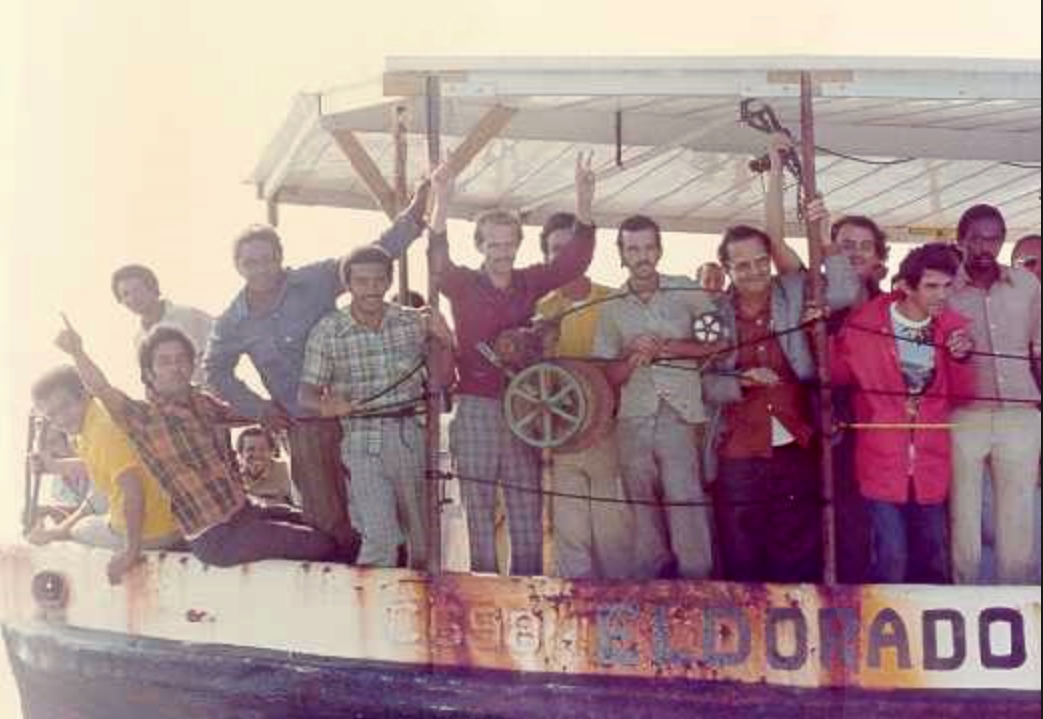
\includegraphics[scale=0.25]{./lecture_includes/boatlift2.png}
	\end{figure}
\end{frame}

\begin{frame}[plain]
	\begin{figure}
	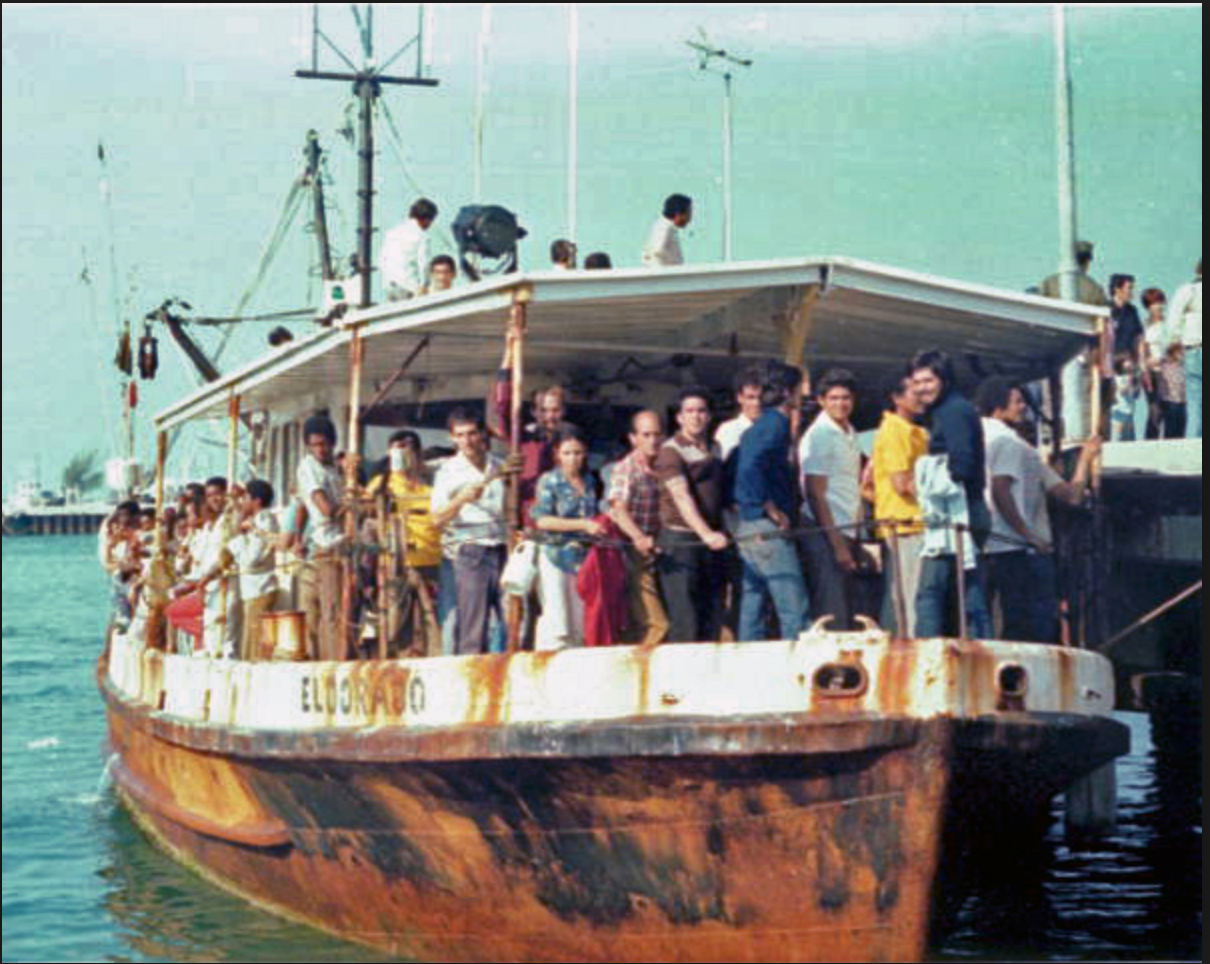
\includegraphics[scale=0.25]{./lecture_includes/boatlift3.png}
	\end{figure}
\end{frame}

\begin{frame}[plain]
	\begin{figure}
	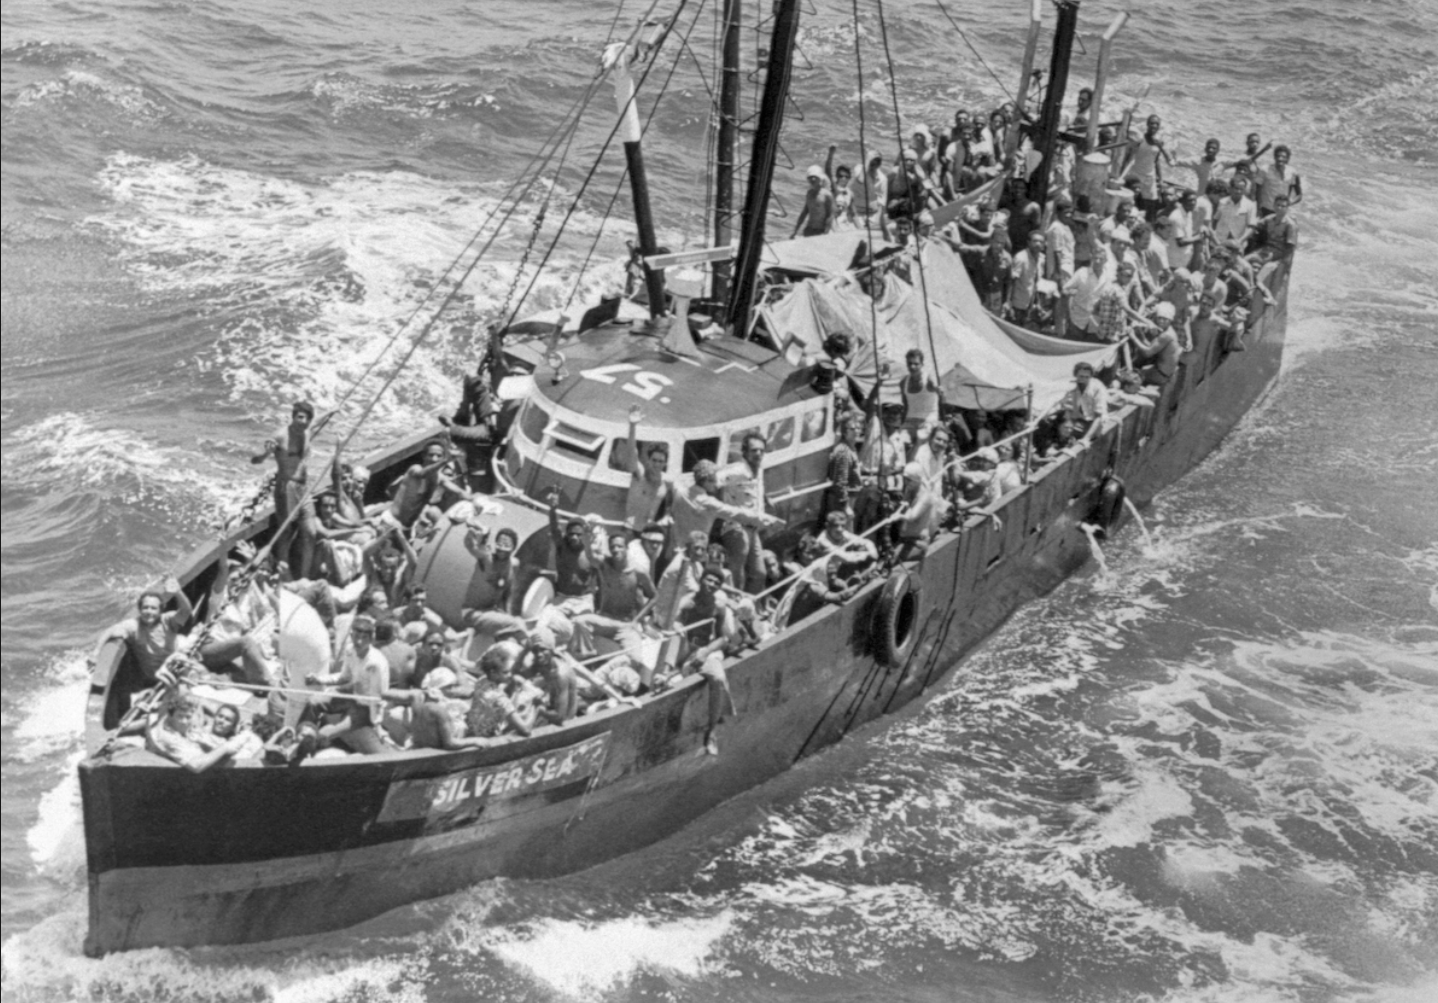
\includegraphics[scale=0.25]{./lecture_includes/boatlift4.png}
	\end{figure}
\end{frame}




\begin{frame}{Description of the Mariel Boatlift}
	
	\begin{itemize}
	\item Fidel Castro said native Cubans could leave permanently so long as they did in late 1980 from Mariel boat dock (``Mariel Boatlift'')
	\item Mariel Boatlift took 100,000 to Miami causing Miami labor force to increase by 7\%
	\item Card (1990) uses the Mariel Boatlift of 1980 as a natural experiment to measure the causal effect of a sudden influx of immigrants on unemployment among less-skilled natives -- finds no effect leading to controversy to a degree
	\item Individual-level unemployment from the Current Population Survey (CPS) for Miami and four selected comparison cities: Atlanta, Los Angeles, Houston, Tampa-St. Petersburg
	\end{itemize}
\end{frame}


\begin{frame}{Why Atlanta, Los Angeles, Houston, Tampa-St. Petersburg?}

	\begin{figure}
	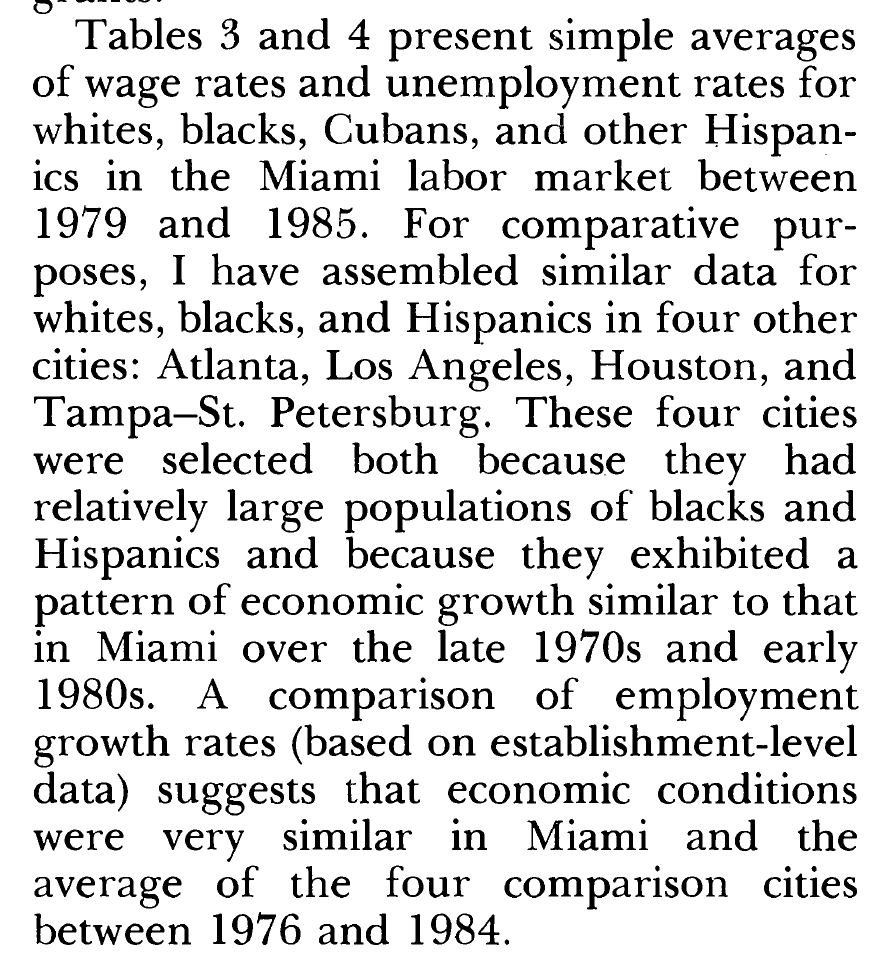
\includegraphics[scale=0.25]{./lecture_includes/card_illr.png}
	\end{figure}

\end{frame}

\begin{frame}{Card's main results}
	
	\begin{figure}
	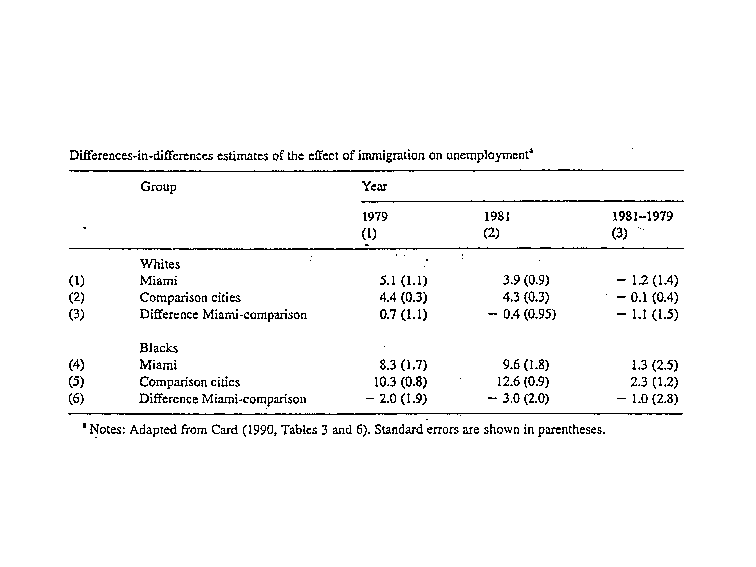
\includegraphics[scale=0.75]{./lecture_includes/abadie_2.pdf}
	\end{figure}
\end{frame}

\begin{frame}{Abadie and synthetic control}

\begin{itemize}
\item Synthetic control was developed by Alberto Abadie (then a grad student, now MIT professor) as a way to do causal inference that didn't ``cherry pick'' control groups while also minimizing selection bias
\item Basic idea: create an ``optimally'' weighted comparison group that recreates the flow of outcomes beforehand and use those weights to predict the post counterfactual to estimate ATT
\item Abadie and Gardeazabal (2003) is a study of a terrorist attack using optimally weighted Spanish regions as comparison for Basque (2010 JASA with new coauthors reintroduces it)
\end{itemize}
\end{frame}


\begin{frame}{Researcher's objectives}

\begin{itemize}
	\item Predict counterfactual of a treated unit post-treatment with imputation by matching on covariates and lagged outcomes prior to the intervention
	\item ``Matching'' will mean here to find weights that minimize the difference between a matrix of treatment group covariates and donor pool covariates
	\item Those weights will be ``optimal'' because they minimized the difference in the observables
	\item Weights are then applied to outcomes to create an alternative timeline of what would have happened had the treatment not occurred (called the ``synthetic control'')
\end{itemize}

\end{frame}

\begin{frame}{Advantages of synthetic control}
	
	\begin{itemize}
	\item Precludes extrapolation (unlike regression) because the imputed counterfactual is based on actual units' real data, not functional form
	\item Weights are calculated so we know exactly what each unit (e.g., state) contributes to the synthetic control
	\item Formalizing the way comparison units are chosen has direct implications for inference
	\end{itemize}
\end{frame}


\begin{frame}{Synthetic control method: estimation}
	
Suppose that we observe $J+1$ units in periods $1, 2, \dots, T$
		\begin{itemize}
		\item Unit ``one'' is exposed to the intervention of interest (that is, ``treated'') during periods $T_0+1, \dots, T$
		\item The remaining $J$ are an untreated reservoir of potential controls (a ``donor pool'')
		\end{itemize}	
\end{frame}


\begin{frame}{Potential outcomes notation}

Define potential outcomes and realized outcomes:

		\begin{itemize}
		\item Let $Y_{it}^0$ be the outcome that would be observed for unit $i$ at time $t$ in the absence of the intervention
		\item Let $Y_{it}^1$ be the outcome that would be observed for unit $i$ at time $t$ if unit $i$ is exposed to the intervention in periods $T_0+1$ to $T$.
		\end{itemize}

\begin{eqnarray*}
\delta_{1t}&=&Y_{1t}^1 - Y_{1t}^0 \\
&=& Y_{1t} - Y_{1t}^0 
\end{eqnarray*} for each post-treatment period, $t>T_0$ and $Y_{1t}$ is the outcome for unit one at time $t$. We will estimate $Y^0_{1t}$ using the $J$ units in the donor pool 

\end{frame}


\begin{frame}{Estimating optimal weights}
	
	\begin{itemize}
	\item Let $W=(w_2, \dots, w_{J+1})'$ with $w_j\geq 0$ for $j=2, \dots, J+1$ and $w_2+\dots+w_{j+1}=1$. Each value of $W$ represents a potential synthetic control
	\item Let $X_1$ be a $(k\times 1)$ vector of pre-intervention characteristics for the treated unit.  Similarly, let $X_0$ be a $(k\times J)$ matrix which contains the same variables for the unaffected units.
	\item The vector $W^*=(w_2^*, \dots, w_{J+1}^*)'$ is chosen to minimize $||X_1-X_0W||$, subject to our weight constraints
	\end{itemize}
\end{frame}

\begin{frame}{Optimal weights differ by another weighting matrix}
	
Abadie, et al. consider $$||X_1 - X_0W||=\sqrt{(X_1-X_0W)'V(X_1-X_0W)}$$where $X_{jm}$ is the value of the $m$-th covariates for unit $j$ and $V$ is some $(k\times k)$ symmetric and positive semidefinite matrix

\end{frame}

\begin{frame}{More on the V matrix}

Typically, $V$ is diagonal with main diagonal $v_1, \dots, v_k$.  Then, the synthetic control weights $w_2^*, \dots, w_{J+1}^*$ minimize: $$\sum_{m=1}^k v_m \bigg(X_{1m} - \sum_{j=2}^{J+1}w_jX_{jm}\bigg)^2$$ where $v_m$ is a weight that reflects the relative importance that we assign to the $m$-th variable when we measure the discrepancy between the treated unit and the synthetic controls

\end{frame}

\begin{frame}{Choice of $V$ is critical}
	
		\begin{itemize}
		\item The synthetic control $W^*(V^*)$ is meant to reproduce the behavior of the outcome variable for the treated unit in the absence of the treatment
		\item Therefore, the $V^*$ weights directly shape $W^*$
		\end{itemize}
\end{frame}

\begin{frame}{Estimating the $V$ matrix}
	
 Choice of $v_1, \dots, v_k$ can be based on
		\begin{itemize}
		\item Assess the predictive power of the covariates using regression
		\item Subjectively assess the predictive power of each of the covariates, or calibration inspecting how different values for $v_1, \dots, v_k$ affect the discrepancies between the treated unit and the synthetic control
		\item Minimize mean square prediction error (MSPE) for the pre-treatment period (default):
			\begin{eqnarray*}
			\sum_{t=1}^{T_0} \bigg(Y_{1t} - \sum_{j=2}^J w_j^*(V^*)Y_{jt} \bigg)^2
			\end{eqnarray*}
		\end{itemize}
\end{frame}

\begin{frame}{Cross validation}

\begin{itemize}
		\item Divide the pre-treatment period into an initial \textbf{training} period and a subsequent \textbf{validation} period
		\item For any given $V$, calculate $W^*(V)$ in the training period.
		\item Minimize the MSPE of $W^*(V)$ in the validation period
\end{itemize}

\end{frame}


\begin{frame}{Suppose $Y^0$ is given by a factor model}

Recall that difference-in-differences used the parallel trends assumption:  $E[\Delta Y^0|D=1]=E[\Delta Y^0|D=0]$, but synth allows for nonlinearities (but still must be modeled)

\bigskip

What about unmeasured factors affecting the outcome variables as well as heterogeneity in the effect of observed and unobserved factors?
\begin{eqnarray*}
Y_{it}^0 = \alpha_t + \theta_t Z_i + \lambda_t u_i + \varepsilon_{it}
\end{eqnarray*}where $\alpha_t$ is an unknown common factor with constant factor loadings across units, and $\lambda_t$ is a vector of unobserved common factors

\end{frame}

\begin{frame}{What makes a good model?}

You are not using parallel trends, but rather your ability to model the movement of your treatment group over a long period of time.

\bigskip

This method is data hungry, less so on the number of units than on the amount of data \emph{pre-treatment}

\bigskip

You may need 15 to 20 years pre-treatment, minimum (we used 43 years) because you need to find a weighted average that goes through all the ups and downs as your treatment group


\end{frame}


\begin{frame}{Example: California's Proposition 99}
	
	\begin{itemize}
	\item In 1988, California first passed comprehensive tobacco control legislation:
		\begin{itemize}
		\item increased cigarette tax by 25 cents/pack
		\item earmarked tax revenues to health and anti-smoking budgets
		\item funded anti-smoking media campaigns
		\item spurred clean-air ordinances throughout the state
		\item produced more than \$100 million per year in anti-tobacco projects
		\end{itemize}
	\item Other states that subsequently passed control programs are excluded from donor pool of controls (AK, AZ, FL, HI, MA, MD, MI, NJ, OR, WA, DC)
	\end{itemize}
\end{frame}

\begin{frame}{Cigarette Consumption: CA and the Rest of the US}
	
	\begin{figure}
	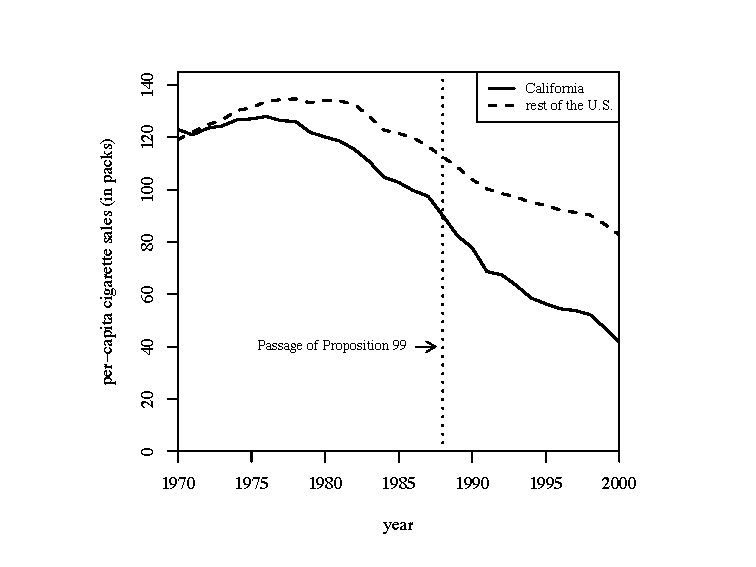
\includegraphics[scale=0.75]{./lecture_includes/abadie_3.pdf}
	\end{figure}
\end{frame}

\begin{frame}{Cigarette Consumption: CA and synthetic CA}
	
	\begin{figure}
	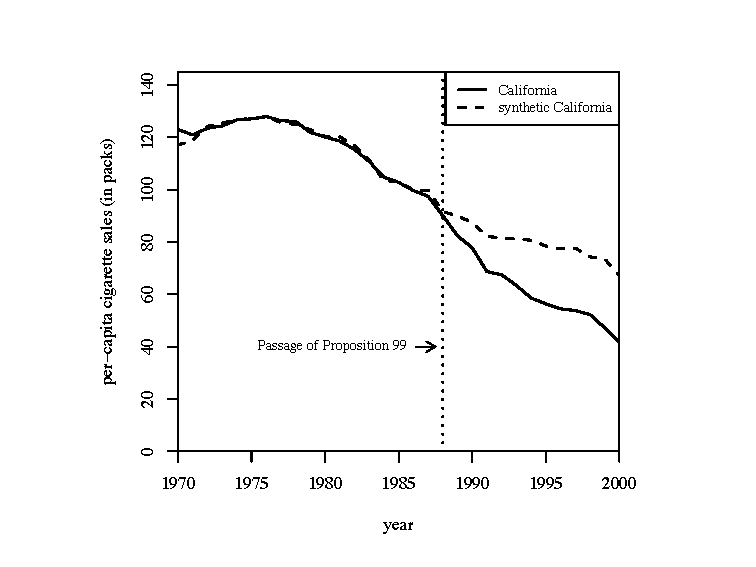
\includegraphics[scale=0.75]{./lecture_includes/abadie_4.pdf}
	\end{figure}
\end{frame}

\begin{frame}{Predictor Means: Actual vs. Synthetic California}
	
	\begin{figure}
	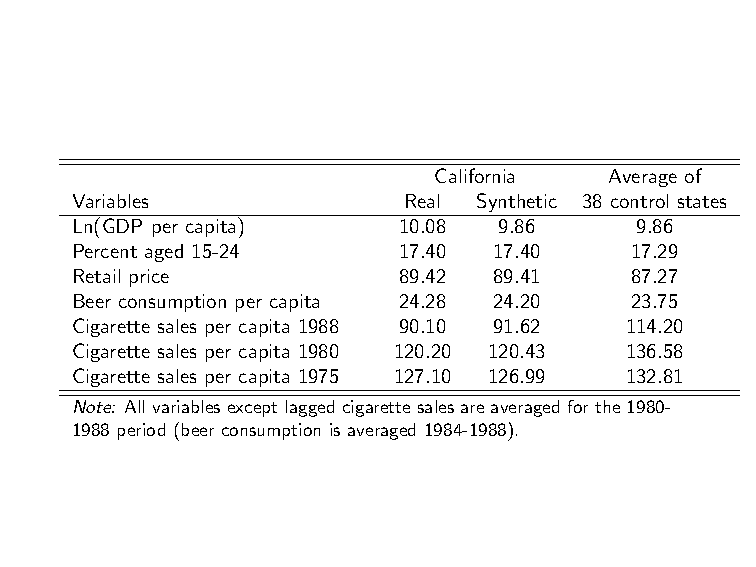
\includegraphics[scale=0.75]{./lecture_includes/abadie_5.pdf}
	\end{figure}
\end{frame}

\begin{frame}{Smoking Gap between CA and synthetic CA}
	
	\begin{figure}
	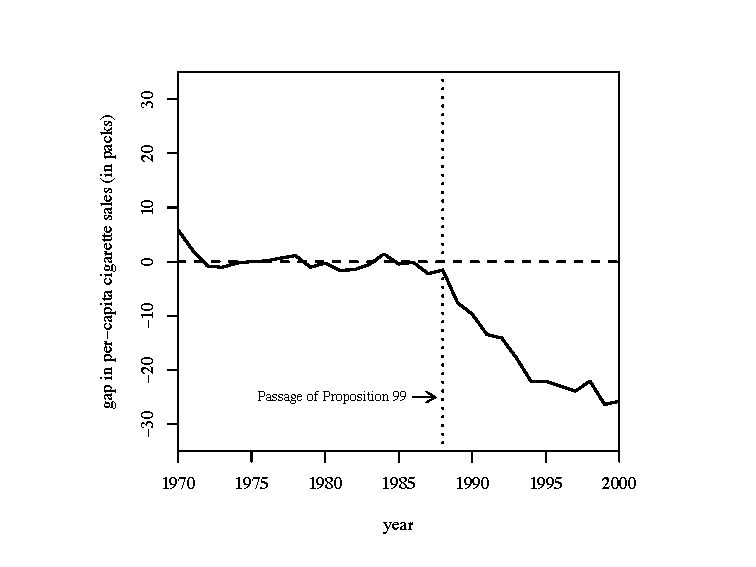
\includegraphics[scale=0.75]{./lecture_includes/abadie_6.pdf}
	\end{figure}
\end{frame}

\begin{frame}{Inference}
	
	\begin{itemize}
	\item To assess significance, we calculate exact p-values under Fisher's sharp null using a test statistic equal to after to before ratio of RMSPE
	\item Exact p-value method
		\begin{itemize}
		\item Iteratively apply the synthetic method to each country/state in the donor pool and obtain a distribution of placebo effects
		\item Compare the gap (RMSPE) for California to the distribution of the placebo gaps. For example the post-Prop. 99 RMSPE is: 
			\begin{eqnarray*}
			RMSPE = \bigg(\frac{1}{T-T_0} \sum_{t=T_0+1}^T \bigg(Y_{1t} - \sum_{j=2}^{J+1} w_j^* Y_{jt}\bigg)^2 \bigg)^{\frac{1}{2}}
			\end{eqnarray*}and the exact p-value is the treatment unit rank divided by $J$
		\end{itemize}
	\end{itemize}
\end{frame}

\begin{frame}{Smoking Gap for CA and 38 control states}
	
	\begin{figure}
	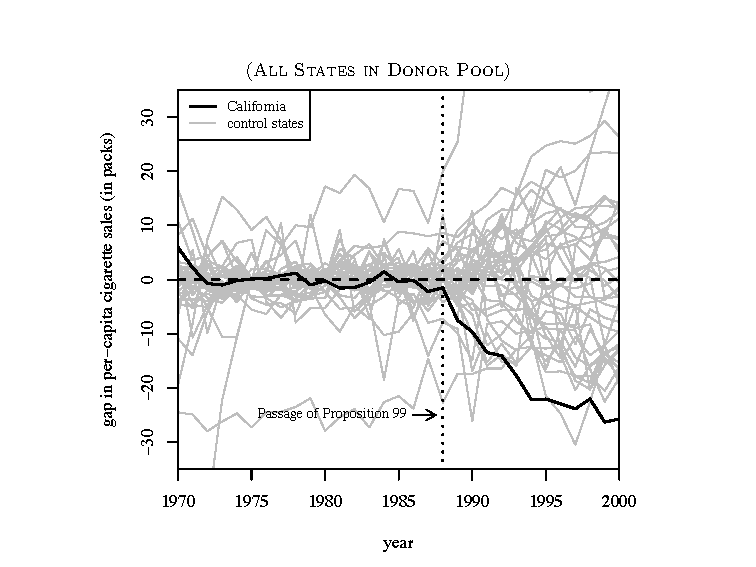
\includegraphics[scale=0.75]{./lecture_includes/abadie_7.pdf}
	\end{figure}
\end{frame}

\begin{frame}{Smoking Gap for CA and 34 control states}
	
	\begin{figure}
	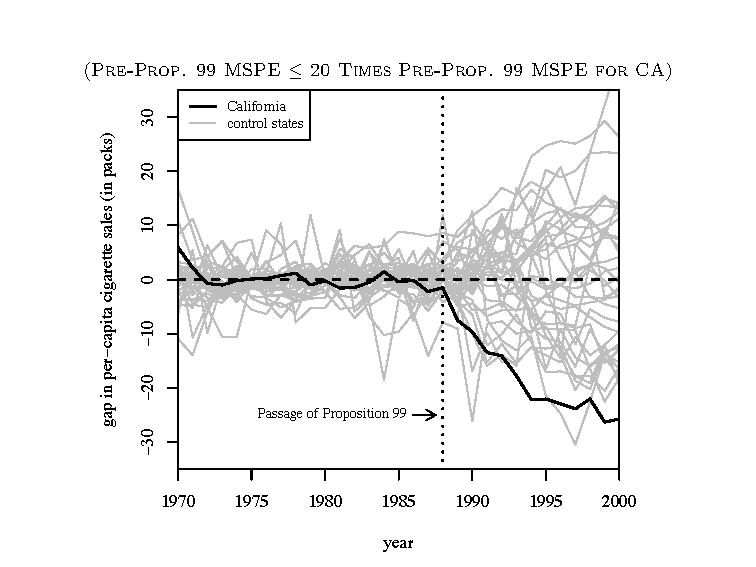
\includegraphics[scale=0.75]{./lecture_includes/abadie_8.pdf}
	\end{figure}
\end{frame}

\begin{frame}{Smoking Gap for CA and 29 control states}
	
	\begin{figure}
	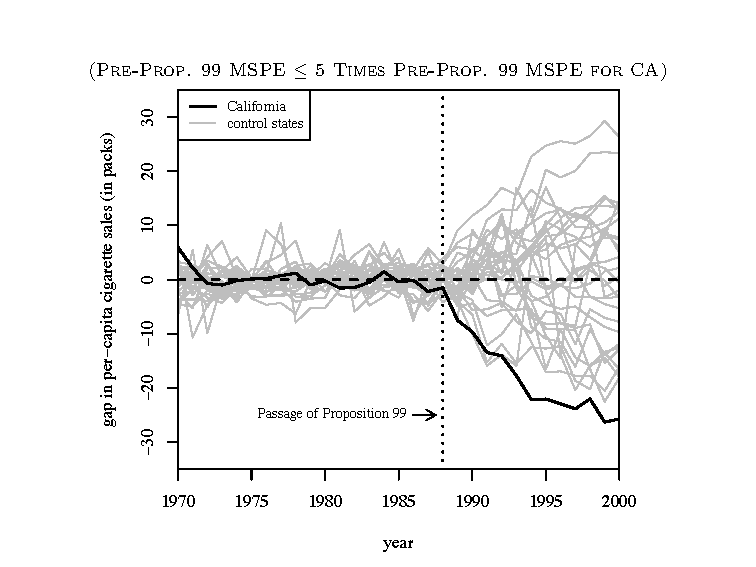
\includegraphics[scale=0.75]{./lecture_includes/abadie_9.pdf}
	\end{figure}
\end{frame}

\begin{frame}{Smoking Gap for CA and 19 control states}
	
	\begin{figure}
	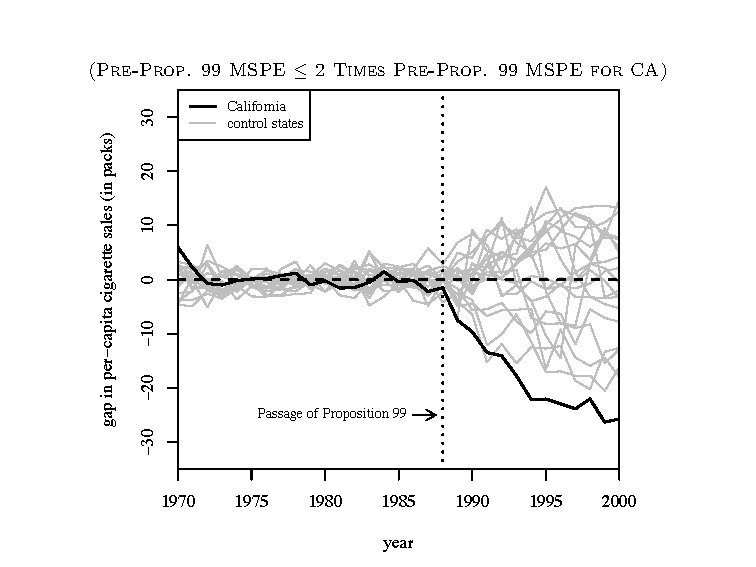
\includegraphics[scale=0.75]{./lecture_includes/abadie_10.pdf}
	\end{figure}
\end{frame}

\begin{frame}{Ratio Post-Prop. 99 RMSPE to Pre-Prop. 99 RMSPE}

	\begin{figure}
	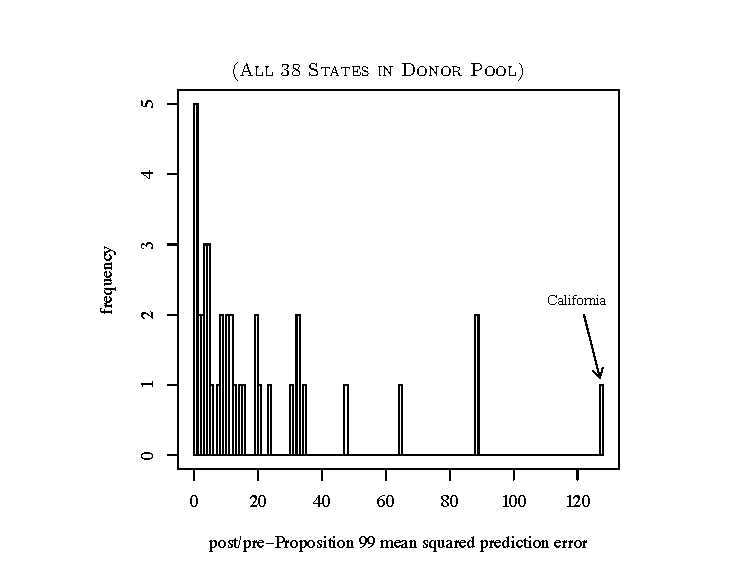
\includegraphics[scale=0.75]{./lecture_includes/abadie_11.pdf}
	\end{figure}
\end{frame}




\begin{frame}{Coding exercise}
	
	\begin{itemize}
	\item The US has the highest prison population of any OECD country in the world 
	\item 2.1 million are currently incarcerated in US federal and state prisons and county jails
	\item Another 4.75 million are on parole
	\item From the early 1970s to the present, incarceration and prison admission rates quintupled in size
	\end{itemize}
\end{frame}



\begin{frame}[plain]

\begin{figure}
\includegraphics[scale=0.5]{./lecture_includes/cook2010.pdf}
\end{figure}
\end{frame}



\begin{frame}{Texas litigation}

	
	\begin{itemize}
	\item Prisons are and have been at capacity for a long time and Texas was overcrowding.  
	\item Ruiz v. Estelle 1980  
		\begin{itemize}
		\item Class action lawsuit against TX Dept of Corrections (Estelle, warden). 
		\item TDC lost.  Lengthy period of appeals and legal decrees.  
		\item Lengthy period of time relying on paroles to manage flows
		\end{itemize}
	\end{itemize}
\end{frame}

\begin{frame}{Prison constraints}

	
	\begin{itemize}
	\item Texas must comply, but faces a problem -- they do not have any capacity
	\item Requires managing ongoing rising flows requires manipulating one of the following
		\begin{itemize}
		\item Prison construction
		\item Overcrowding
		\item Paroles
		\end{itemize}
	\item They intensively parole with very little prison construction until 1993
	\end{itemize}
\end{frame}



\begin{frame}{Texas prison construction}

	
	\begin{itemize}
	\item Governor Ann Richards (D) 1991-1995
		\begin{itemize}
		\item Operation prison capacity increased 30-35\% in 1993, 1994 and 1995. 
		\item Prison capacity increased from 55,000 in 1992 to 130,000 in 1995.  
		\item Building of new prisons (private and public)
		\end{itemize} 
	\end{itemize}
\end{frame}

\begin{frame}[shrink=30,plain]

\begin{figure}
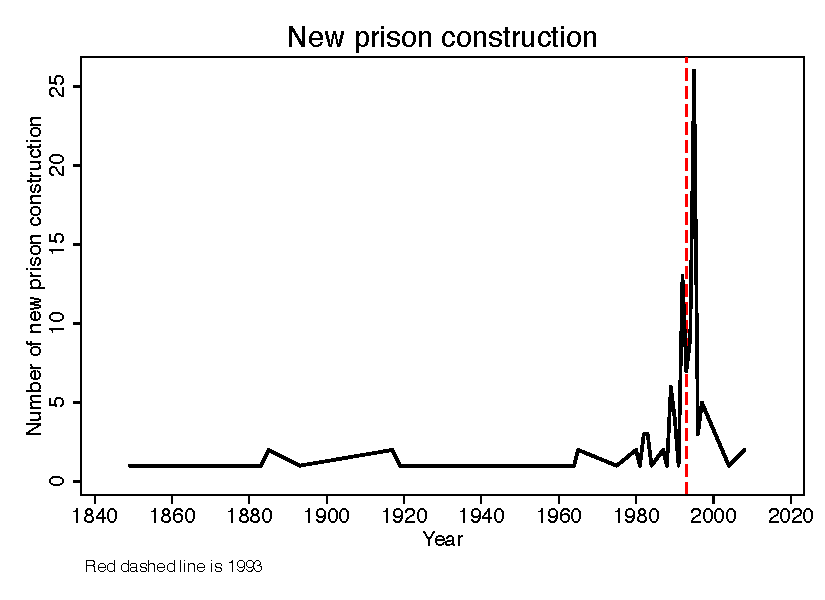
\includegraphics{./lecture_includes/tdcj.pdf}
\end{figure}
\end{frame}


\begin{frame}[shrink=30,plain]
\begin{figure}
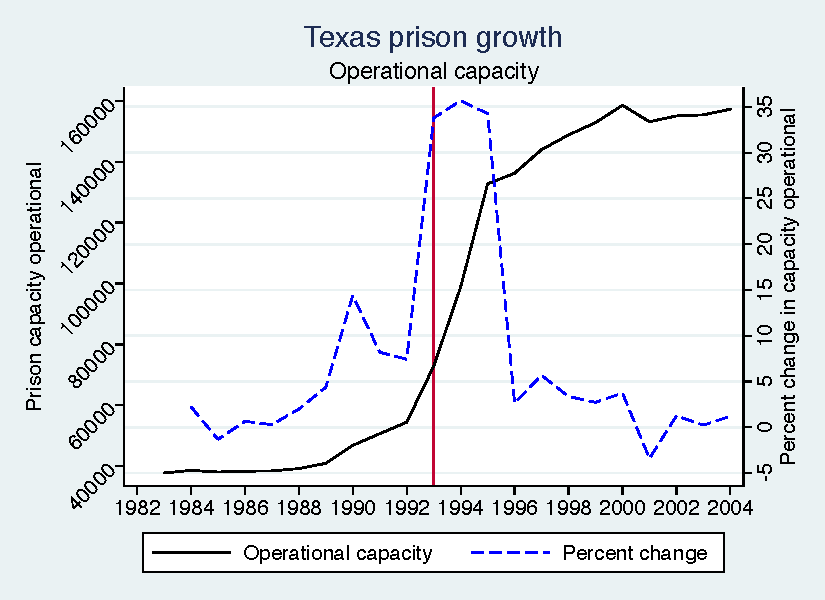
\includegraphics{./lecture_includes/capacity_operational_texas.pdf}
\end{figure}
\end{frame}


\begin{frame}[shrink=30,plain]

\begin{figure}
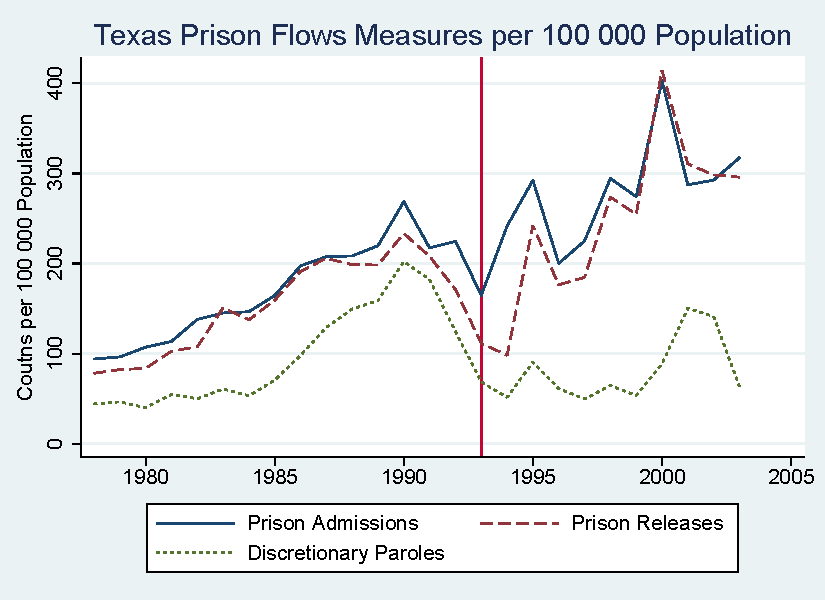
\includegraphics{./lecture_includes/flow_rate_figure.pdf}
\end{figure}
\end{frame}

\begin{frame}[shrink=30,plain]

\begin{figure}
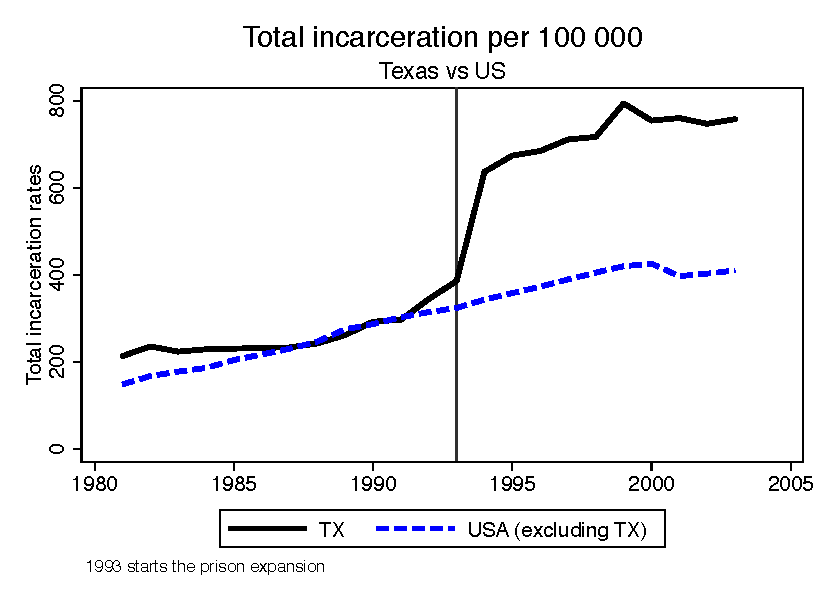
\includegraphics{./lecture_includes/total_incarceration.pdf}
\end{figure}
\end{frame}


\begin{frame}[shrink=30,plain]

\begin{figure}
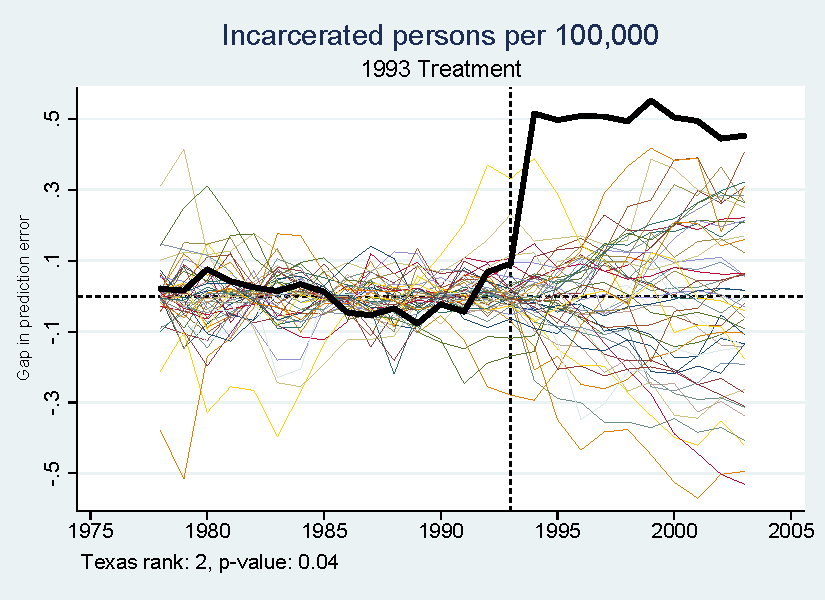
\includegraphics{./lecture_includes/synth_placebo_totalincarceration1993.pdf}
\end{figure}
\end{frame}

\subsection{Event studies in finance}

\begin{frame}{Possibilities for detecting corruption}

\begin{itemize}

\item Event studies in finance have been used to detect abnormal patterns around ``events'' involving single firms
\item Baker and Gelbach (2020) proposes a type of synthetic control estimator that uses machine learning to estimate a counterfactual, as opposed to imposing strong parametric assumptions
\item Examples of its use have been applied to disruptions with the Elon Musk Twitter deal which while not corruption does involve estimating potential damages from stock price movements

\end{itemize}

\end{frame}

\begin{frame}{Largest Securities Class Action Settlements}

\begin{enumerate}

\item Enron: \$7.2b
\item WorldCom Inc: \$6.1b
\item Tyco International Ltd.: \$3.2b
\item Cendant Corporation: \$3.2b

\end{enumerate}

\end{frame}

\begin{frame}{Over time}

\begin{figure}
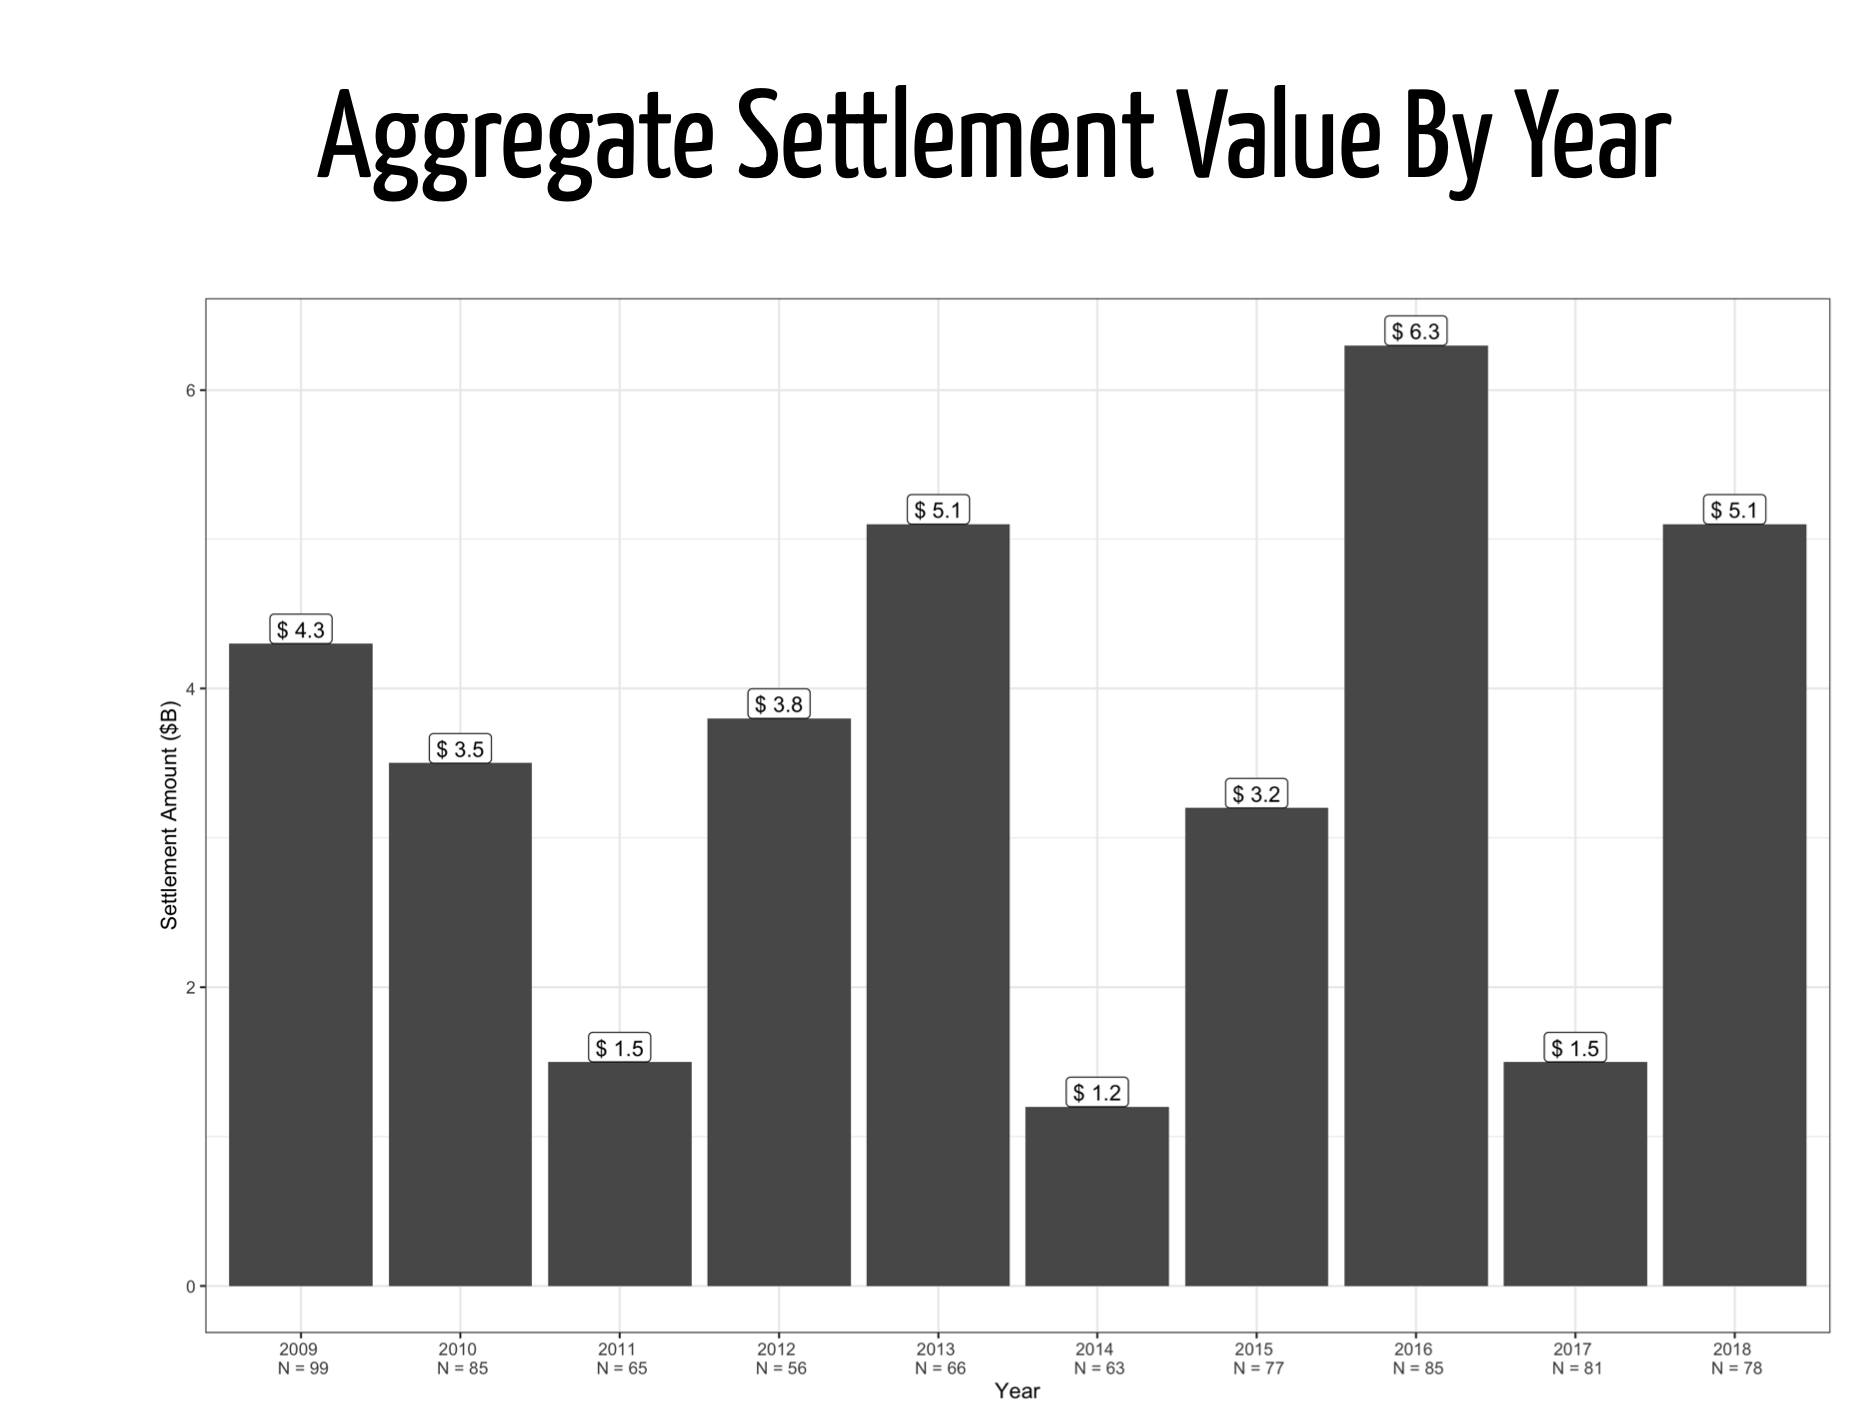
\includegraphics[scale=0.35]{./lecture_includes/baker_gelbach_1}
\end{figure}
\end{frame}

\begin{frame}{Event studies and securities litigation}

\begin{itemize}

\item Historically, the ``event study'' estimated ``abnormal'' returns under strong parametric assumptions (e.g., normality), but non-normal returns are normal

\begin{quote}
``The abnormal returns are the parameters that determine the damage estimates in securities suits, it is worthwhile to explore whether methods exist that can provide more accurate estimates of the abnormal return itself.''
\end{quote}

\item They argue that the event study is an out-of-sample prediction problem, which ML is used for, but it is also an extension of the synth modeling framework

\end{itemize}

\end{frame}

\begin{frame}{Basic idea}

\begin{figure}
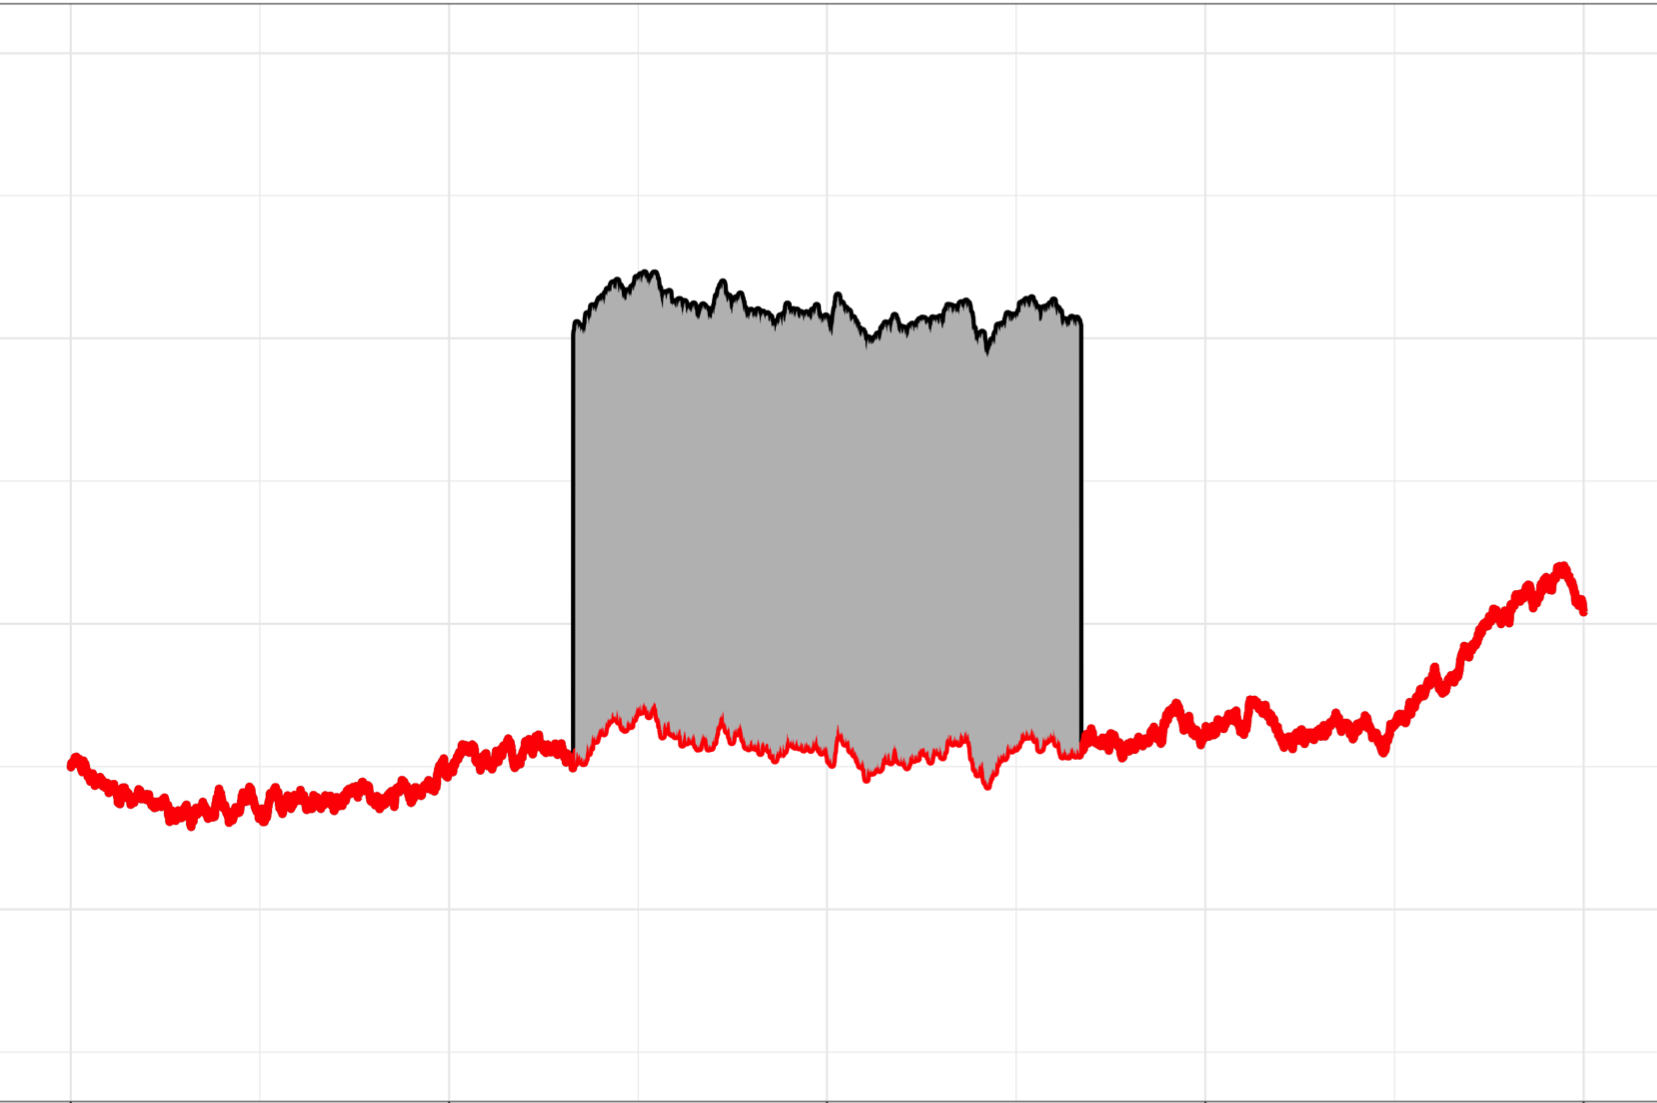
\includegraphics[scale=0.35]{./lecture_includes/baker_gelbach_2}
\end{figure}
\end{frame}


\begin{frame}{Event studies as a prediction problem}

\begin{itemize}
\item Let the daily return for firm $i$ on date $t$ be $r_{i,t}$ and variables used for prediction is $X_{i,t}$ (e.g., market return, Fama-French and Carhart factors, a 1 for intercept, etc.)
\item Suppose an event reveals fraud.  It's effect on daily return is $r^1_{i,t} - r^0_{i,t}$ and we want to estimate $r^0_{i,t}$ with $\widehat{r}^0_{i,t}$
\item Construct a predicted residual as $\widehat{\varepsilon}_{i,t} = r_{i,t} - \widehat{r}^0_{i,t}$
\item Typically people would estimate this with OLS $$r_{i,t} = \alpha + \beta_1 X_{i,t} + \varepsilon_{i,t}$$
\end{itemize}

\end{frame}

\begin{frame}{OLS, ML, MSE, Bias, Variance}

\begin{itemize}
\item MSE of predicted abnormal return for $\widehat{\varepsilon}_{i,t} = r_{i,t} - \widehat{\beta}X_{i,t}$ is the sum of a squared bias term and a variance term
\item It's possible that the variance of one specification is lower enough than another to make up for a difference in bias
\item OLS also suffers because it overfits data when used for prediction -- it is best unbiased linear predictor but at the price of greater out-of-sample variance linear prediction
\item Since MSE is the basis for measuring prediction accuracy, ML estimators may outperform conventional OLS as we can explore increasing bias and reducing variance
\item ML methods accept bias in exchange for reduced variance out-of-sample accomplished through ``training''
\end{itemize}

\end{frame}

\begin{frame}{Paper's punchline}

\begin{quote}
``Using real stock return data, we demonstrate that a number of out-of-the-box statistical approaches that are relatively easy to interpret perform better than the standard, OLS-based event study specifications used in court proceedings.

\bigskip

We find that specifications using penalized regression generally perform well.  Specifications that adjust for daily market performance using data-driven peer indexes also generally perform well.

\bigskip

Finally, we obtain generally good performance from specifications that use a cross-validation technique that is robust to otherwise unmodeled time-series properties of the DGP. The best specifications provide noticeable improvements over event study approaches conventionally used in securities litigation. 

\end{quote}

\end{frame}

\begin{frame}{Peer index}

\begin{itemize}
\item They note that the best-performing specification makes use of both penalized regression and data-driven peer firm choice.
\item They call this the ``reasonable peer index'', and they show that ML methods can usefully serve as a basis for choosing \emph{which} peer firms to include in an event study (again, making this a synth-like method) which can mitigate the subjective researcher bias that synth is meant to overcome
\item Rather than subjectively picking which firms represent the counterfactual (over which there can be debate clearly, some disingenuous given the amount of money at stake), they propose letting the data say who the best peer is
\item But using \emph{any} peer index appears to mitigate this too
\end{itemize}

\end{frame}

\begin{frame}{Ranking all the ML methods}

\begin{figure}
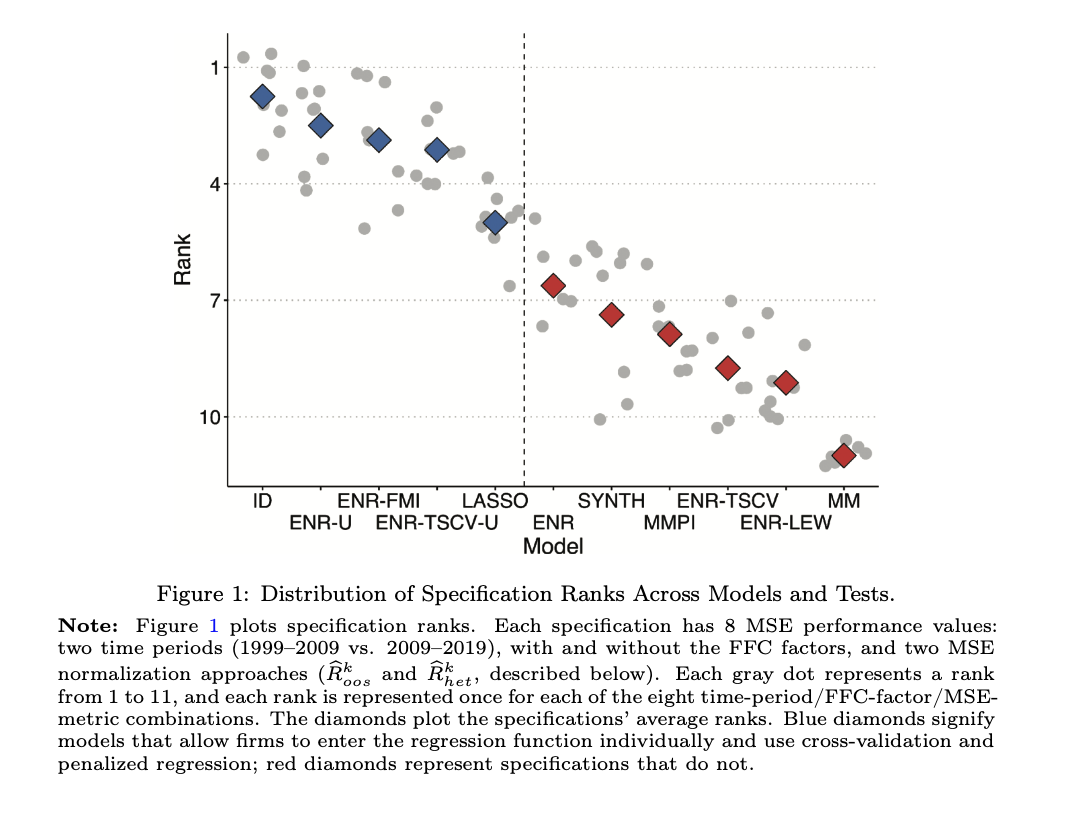
\includegraphics[scale=0.35]{./lecture_includes/baker_gelbach_5}
\end{figure}
\end{frame}

\begin{frame}{Elon Musk example}

\begin{itemize}
\item In an unpublished analysis, Baker examined Elon Musk's attempt to buy Twitter on Twitter's stock price
\item Unlike his published paper, he's only going to use one form of ``penalized'' machine learning called ridge regression (which constrains what the coefficients can be in his model)
\item He will use peer index and the S\&P500 for prediction purposes
\end{itemize}

\end{frame}

\begin{frame}{Purpose of the exercise}

\begin{quote}
``The goal here is to get a rough estimate of what TWTR would be trading at had Elon never put the stock in play. Note, this does not mean that the prediction is equivalent to what TWTR would trade at were the deal to not go through (without any damage payments), as Elon has likely destroyed value in the process. This prediction could in fact be used as a baseline price in any tort-type damages claim that the company would want to bring against Elon after the process is over.''
\end{quote}

\end{frame}

\begin{frame}{Basic idea}

\begin{figure}
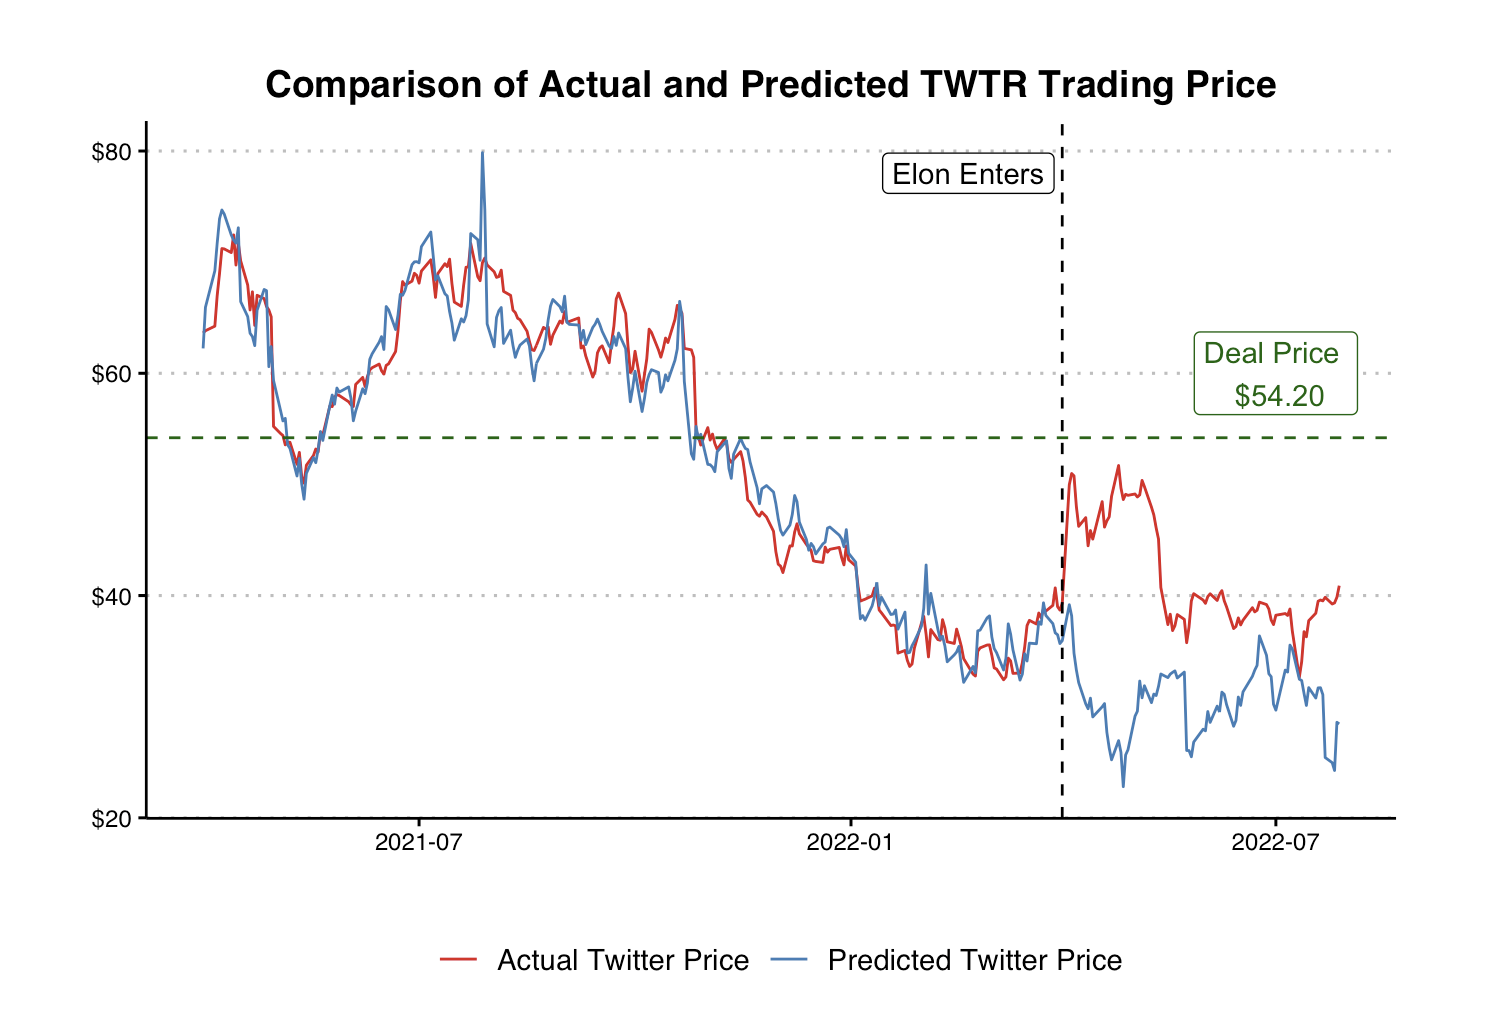
\includegraphics[scale=0.35]{./lecture_includes/baker_gelbach_3}
\end{figure}
\end{frame}

\begin{frame}{Basic idea}

\begin{figure}
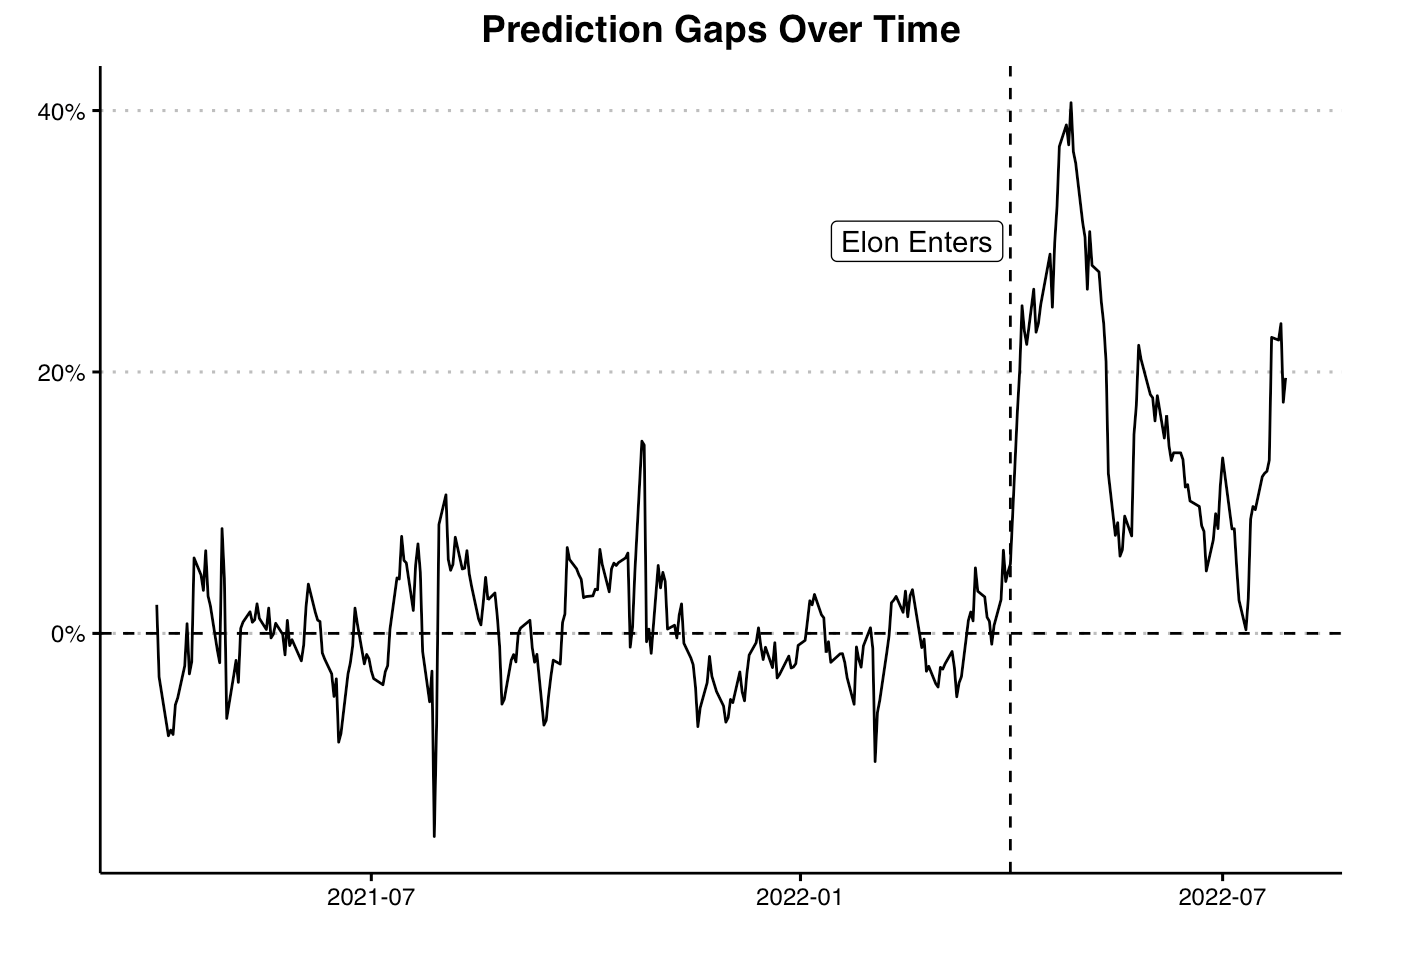
\includegraphics[scale=0.35]{./lecture_includes/baker_gelbach_4}
\end{figure}
\end{frame}

\section{Concluding remarks}

\begin{frame}{Summarizing}

\begin{itemize}
\item Randomized treatments are great but not always available 
\item Causal inference methods can utilize naturally occurring variation, but still must make adequate adjustments to find suitable controls
\item Synthetic control and recent work on event studies can be possibilities
\item Thank you!

\end{itemize}

\end{frame}


\end{document}
